% This is samplepaper.tex, a sample chapter demonstrating the
% LLNCS macro package for Springer Computer Science proceedings;
% Version 2.20 of 2017/10/04
%
\documentclass[runningheads]{llncs}
%
\usepackage{graphicx}
\graphicspath{ {./images/} }
\usepackage{booktabs}
\usepackage{cite}
\usepackage{amsmath,amssymb,amsfonts}
\DeclareMathOperator*{\argmax}{arg\,max}
%\usepackage{algorithmic}
\usepackage{textcomp}
\usepackage{hyperref}
\usepackage{mathptmx}
\usepackage{amssymb}
\usepackage[binary-units=true]{siunitx}
\usepackage{mathtools}
\usepackage[ruled,vlined]{algorithm2e}
\usepackage{amsmath,bm}
\usepackage[utf8]{inputenc}
\usepackage[symbol]{footmisc}
\usepackage{cuted}
\usepackage{subcaption}
\usepackage{placeins}
\usepackage{float}
\usepackage{eso-pic}
\usepackage[normalem]{ulem}
\useunder{\uline}{\ul}{}

\renewcommand{\thefootnote}{\arabic{footnote}}

\begin{document}
%
\title{Lab Vision Systems SS21 \\Stereo Disparity Estimation}
%
\titlerunning{Lab Report SS21}
% If the paper title is too long for the running head, you can set
% an abbreviated paper title here
%
\author{Jan Nogga\inst{1} \and
Fabrice Beaumont\inst{2}}
%
\authorrunning{J. Nogga and F. Beaumont}
% First names are abbreviated in the running head.
% If there are more than two authors, 'et al.' is used.
%
\institute{Universität Bonn, Mat. no. 2663853 \and
Universität Bonn, Mat. no. 2747609}
%
\maketitle              % typeset the header of the contribution
%
\begin{abstract}
Stereo disparity estimation is used to extract depth information from a pair of images.
In this lab report, we implement a simple baseline system for the corresponding supervised learning task. Then, we address its weaknesses and redesign all trainable components to optimize the performance on the KITTI-2015 traffic scene data set. The training process is supported by fine-tuning after pretraining on synthetic samples from the Scene Flow data set. Strong performance is demonstrated and the effects of various aspects of model design and training strategy are discussed in detail.
\end{abstract}
%
%
%


\section{Introduction}
Stereo disparity estimation is the task of finding pixel correspondences and reckoning their distances along one axis, given a pair of stereo images. Since depth is inversely proportional to disparity, such a disparity image is equivalent to a depth image, if the parameters of the imaging rig are known. Naturally, depth information has many applications in different domains, such as object perception in robotics \cite{Object_Perception}, the detection of other traffic participants for autonomous vehicles \cite{Vehicle_Perception} or novel view synthesis in computer graphics \cite{View_Synthesis}. In principle, depth images can also be obtained directly using specialized sensors, such as TOF cameras or LiDAR. These however suffer from the distinct disadvantages that TOF cameras do not perform well in outdoor settings during daytime and LiDAR detectors are costly, while providing only sparse depth maps. On the other hand, stereo imaging rigs require only two cameras, which are comparatively cheap to obtain, and perform well under a variety of lighting conditions, even in darkness. In this case the scene can be illuminated by a separate light source \cite{Light_Source}. Furthermore, many devices natively feature multiple cameras, such as smartphones or even humanoid robots, which often include a camera in each eye socket or are readily extended in this manner. This also applies to the NimbRo-OP2X humanoid robot \cite{NimbRo-OP2X} which we would ultimately like to equip with depth-sensing capabilities on top of already existing perception systems.

In this lab report, we discuss in detail the structure and implementation of a deep disparity estimation framework presented in the course of the lab sessions, referred to in the following as the \textit{baseline model}. Furthermore, we propose improvements to each functional component of the baseline model, implementing a vastly superior system in the process. Next, the effectiveness of different aspects of the training strategy are judged, and the results of our trials illustrated. The final section sketches further steps necessary to apply our work to depth perception for humanoid robots.

\section{Baseline Model}
\begin{figure}[h]
\vspace{-1px}
  \centering
    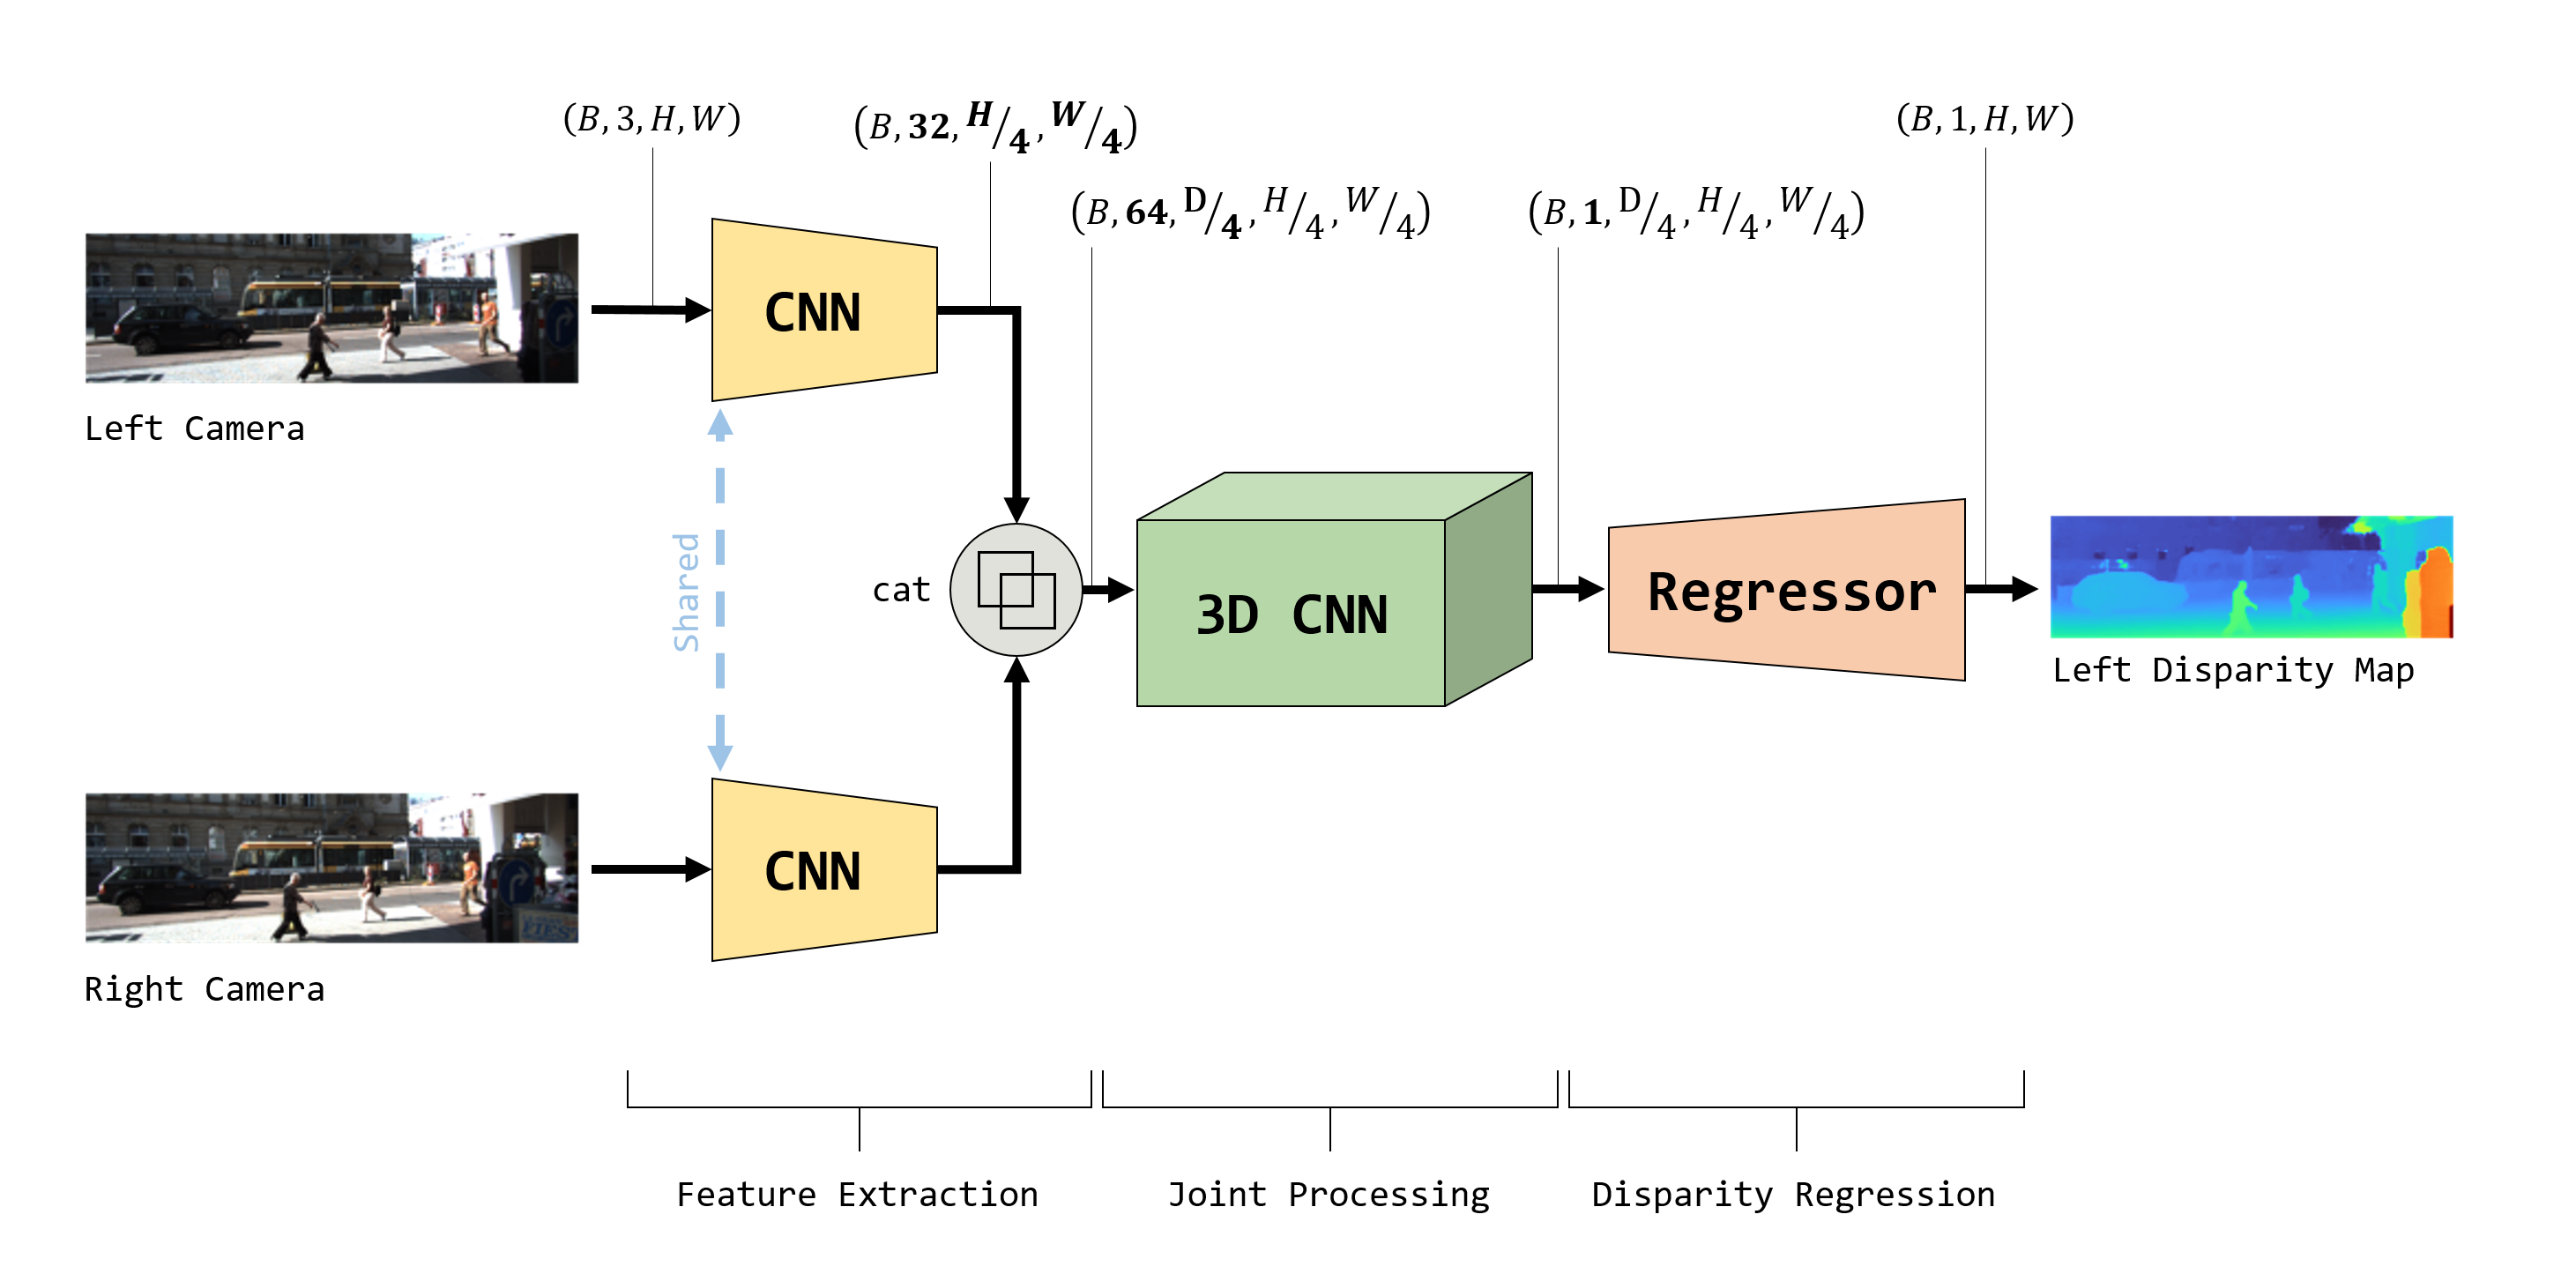
\includegraphics[width=0.99\linewidth]{images/Baseline Model Pipeline.png}
    \caption{An overview of the baseline model.}
    \label{Fig:Baseline_Model_Overview}
\end{figure}
To serve as a reference system for our disparity estimation framework, we implement the baseline model as described in the lab session. It consists of a shared feature extraction network, a joint processing 3D CNN module for left and right features related at different levels of disparity in a cost volume, and finally a regressor that outputs a disparity estimate per pixel. This model is depicted in figure \ref{Fig:Baseline_Model_Overview}.
\subsection{Shared Feature Extraction}
Input images are passed through a shared CNN consisting of eight residual blocks. Each residual block comprises two convolutional layers with batch normalization and a rectified linear unit function (ReLu). They are bypassed by a skip connection which transports the input past the two convolutional layers, adding it to the output of the second batch normalization before the application of the final nonlinearity. If necessary, the skip connection is equipped with one layer of $1 \times 1$-convolution to address potential strides or channel adjustments desired for the respective residual blocks. All other convolutions utilize $3 \times 3$-kernels and corresponding padding. This is the standard layout as described in \cite{ResNet}. Our specific implementation maps the three input channels to $8-8-16-16-16-32-32-32$ output channels, using a convolution with stride $2$ in the first layer of the residual block each time the number of output channels is increased. Since a sensible feature extraction is assumed to be comparable for either left or right input image, both are processed by the same network weights in a Siamese fashion.

\subsection{Concatentation Cost Volume}
The feature maps $f_l$, $f_r$ corresponding to the left and right input images are combined by concatenation across different disparity levels. After the application of the strided residual convolutions in the preceding feature extraction, the feature maps have a reduced spatial dimension of $H'=H/4$ (height), $W'=W/4$ (width). Likewise, the maximum disparity $D$ is reduced to $D'=D/4$, since after all, disparity is measured in pixel coordinates. Specifically, the cost volume $C_{\text{concat}}( \star,d,x,y)$ is created according to the following formula:

\begin{equation}
   C_{\text{concat}}(\star,d,x,y)  = \text{Concat} \{ f_l(x,y), f_r(x-d,y) \}
\end{equation}

Note that the star indicates the dimension in which the $32$ channels of either feature map are concatenated to the $64$ channels of the cost volume. This process is preferable to simply seemingly self-evident alternative of concatenating $f_l$ and $f_r$, because it encodes our understanding of the geometry of disparity estimation. This way downstream modules do not need to uncover this aspect on their own \cite{Cost_Volume}. In our implementation, we adapt code from \cite{GwcGit} and set the maximum disparity to $D=192$.

\subsection{Joint Disparity Processing}\label{Sec:Joint_Processing}
The output of the cost volume is processed by four 3D residual CNN blocks. These represent straightforward generalizations of the previously used 2D residual blocks, simply using 3D instead of 2D convolutions. Their purpose is to take into account local context when processing the cost volume to produce a score per disparity level and spatial location. This architecture for joint processing is common practice in disparity estimation \cite{Cost_Volume}, but usually applies much deeper architectures than four residual blocks. We nonetheless do not increase this number in order to meet the requirements as stated in the lab session. In our implementation, the 3D residual blocks map the $64$ input channels to $32-16-8-1$ output channels.

\subsection{Disparity Regression}
The previous step learns a $1 \times D' \times H' \times W'$ set of disparity scores per pixel. This is upsampled by a factor of four using a nearest neighbor interpolation, following Ocamm's razor as other interpolation methods did not noticeably improve the results. Using the softmax function on the disparity channel, the upsampled volumes are then converted to a probability distribution over possible disparity levels per pixel location. From these distributions, we obtain the expected disparity value as dot product of the probabilities with a template vector containing integer disparities in $[0, D)$. We believe this type of regressor is advantageous because it does not require any trainable parameters. However, it is important to note that the distributions resulting from the softmax step are potentially multi-modal, and in consequence, this type of soft argmax function might not always be a good descriptor of the true disparity. This is addressed in other work, for example by calculating an expectation and shifting it based on the properties of the distribution \cite{Wasserstein_Dist_Disp_Estimation}. Instead, we must rely on the preceding joint processing step to produce adequate scores to that effect.

\section{FF-GwcNet}
\begin{figure}[h]
\vspace{-1px}
  \centering
    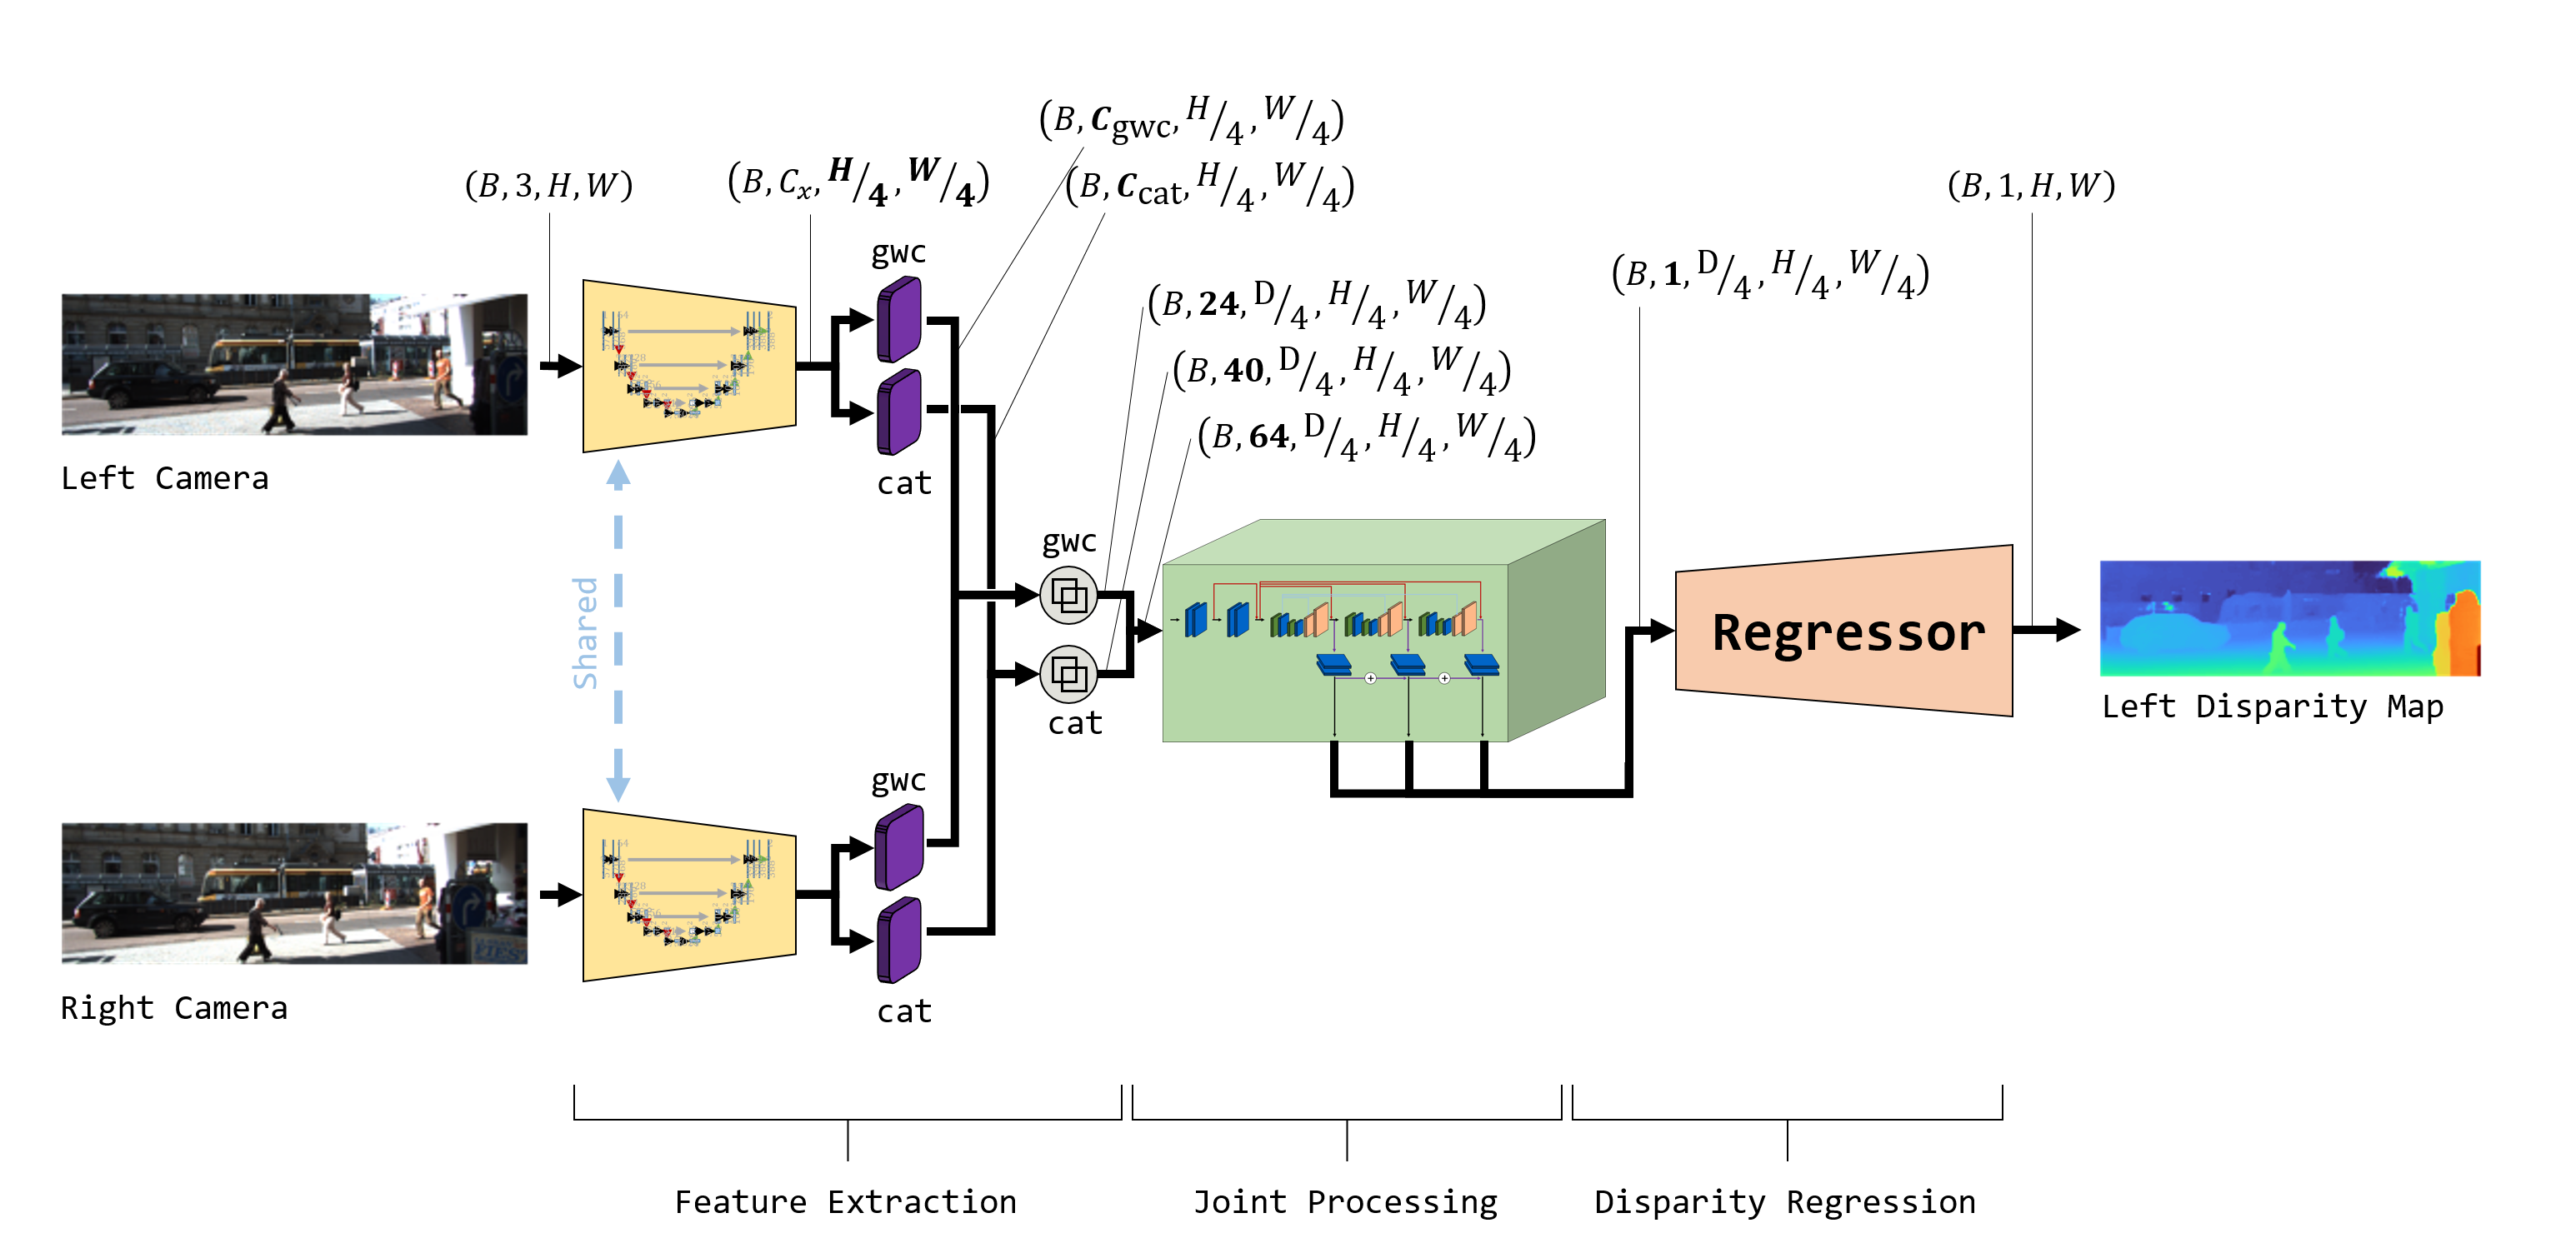
\includegraphics[width=0.99\linewidth]{images/Custom Model Pipeline.png}
    \caption{The architecture of FF-GwcNet.}
    \label{Fig:Custom_Model_Overview}
\end{figure}

With the baseline model in place, we proceed by reexamining its individual components with the intention of maximizing performance. Since the style of its framework, a feature extraction followed by joint processing of a cost volume and a final regression step, has remained unchanged over several generations of disparity estimation systems \cite{Cost_Volume, PSM-Net, guo2019groupwise, Wasserstein_Dist_Disp_Estimation}, we do not attempt to reinvent the wheel. Instead, we apply several targeted changes within the scope of a specific sub-module, ensuring that they reassemble just as before. Therefore, it is sufficient to explain the components individually from left to right, as depicted in figure \ref{Fig:Custom_Model_Overview}.

\subsection{Feature Fusion}\label{Sec:Feature_Fusion}
The baseline model's feature extraction consisted of only a few residual blocks and was thus of limited capacity. However, depth cues can be affected by a multitude of confounders, such as reflections, motion blur, lighting discrepancies or even quite banal reasons such as billboards hosting some imagery present in the scene. We believe that due to the complexity of these challenges, the image features must be as rich as possible, such that hallucinations of depth are less likely to occur. One approach, which would be quickest to implement, would be to replace the feature extraction with the convolutional layers from a pretrained classifcation backbone, which are readily available online. Keeping in mind that our superordinate goal is to produce a model which can be deployed on a humanoid robot, and that we in fact have a U-Net based semantic segmentation model existing in the perception system in our use-case, we decide to go beyond using just the encoder from a classification model. Instead, we attempt what we refer to as \textit{feature fusion}. After each decoder layer of a U-Net, we down- or upsample the resulting feature map to a desired output resolution, in our case $H' \times W'$, cache it, and finally concatenate all of these along the channel dimension. Thus, the feature map per image becomes a $C_x \times H' \times W'$ structure for each sample stereo pair. Here, $C_x=\sum_{i=1}^{depth}C_i$ is the sum of decoder output channels $C_i \in \{256, 128, 64, 32, 16\}$ up to a certain depth which corresponds to the number of stages used in the encoder. Since our feature fusion U-Net arises from some model surgery applied to U-Nets with pretrained encoders from the SMP library \cite{SMP}, encoder depths of $3$ to $5$ are possible. Using models adapted from this library is beneficial, because it provides countless well known encoder backbones with weights pretrained on selected datasets.
%\\TODO: CONTINUE REVIEW
\subsection{Group-wise Correlation Cost Volume}\label{Sec:Gwc}
The concatenation cost volume we employ in the baseline model was proposed to address the problem of feature decimation inherent to the alternative at that time, a correlation cost-volume \cite{Cost_Volume}. This consists simply of the inner product between a feature vector of length $N$ from the left and one from the right frame, while the x-coordinate of the latter is offset by a given disparity level

\begin{equation}
   C_{\text{Corr}}(d,x,y)  = \frac{1}{N} \langle f_l(x,y), f_r(x-d,y)\rangle.
\end{equation}

This is efficient to calculate, but not very expressive, as information stored in the channel dimension is lost. On the other hand, the concatenation cost volumes store many redundant feature channels in a huge data structure. A compromise is given by \textit{group-wise correlation}, where the feature channels are partitioned into $N_g$ sections, and the correlation is calculated between features of each group \cite{guo2019groupwise}. Formally, the group-wise correlation (gwc) cost volume is given by

\begin{equation}
   C_{\text{Gwc}}(g,d,x,y)  = \frac{1}{N / N_g} \langle f_l^g(x,y), f_r^g(x-d,y)\rangle,
\end{equation}

where $f_l^g(x,y)$, $f_r^g(x-d,y)$ refer to segments $g$ of the feature vectors at spatial positions $(x,y)$, $(x-d,y)$ of the left feature map and the disparity-offset right feature map. The length of each of these vectors is $\frac{N}{N_g}$, implying that the number of feature channels input into this structure must be divisible by $N_g$. In our case, we input $160$ channels respectively for the left and right feature maps, and group-wise correlate these using $40$ groups, again using an implementation only slightly adapted from \cite{GwcGit}. It has been demonstrated that, while this type of cost volume is very efficient, small concatenation cost volumes should be utilized in parallel \cite{guo2019groupwise}. Therefore, we also construct a cost volume as for the baseline model, but only using $12$ input and thus $24$ cost volume channels, later concatenating these with the aforementioned gwc cost volume to produce a data structure shaped $64 \times D' \times H' \times W'$ per input sample for subsequent joint processing. Of course, our output from the previous module utilizes $C_x$ channels, so we use one residual block per cost volume type to map them to $160$ and $12$ channels respectively. Negligible computational costs incur for these layers, so we do not share them for left and right feature maps. Instead, we hope to automatically adapt to potential idiosyncrasies of the camera array in this manner.

\subsection{Stacked Hourglass}
\begin{figure}[h]
\vspace{-1px}
  \centering
    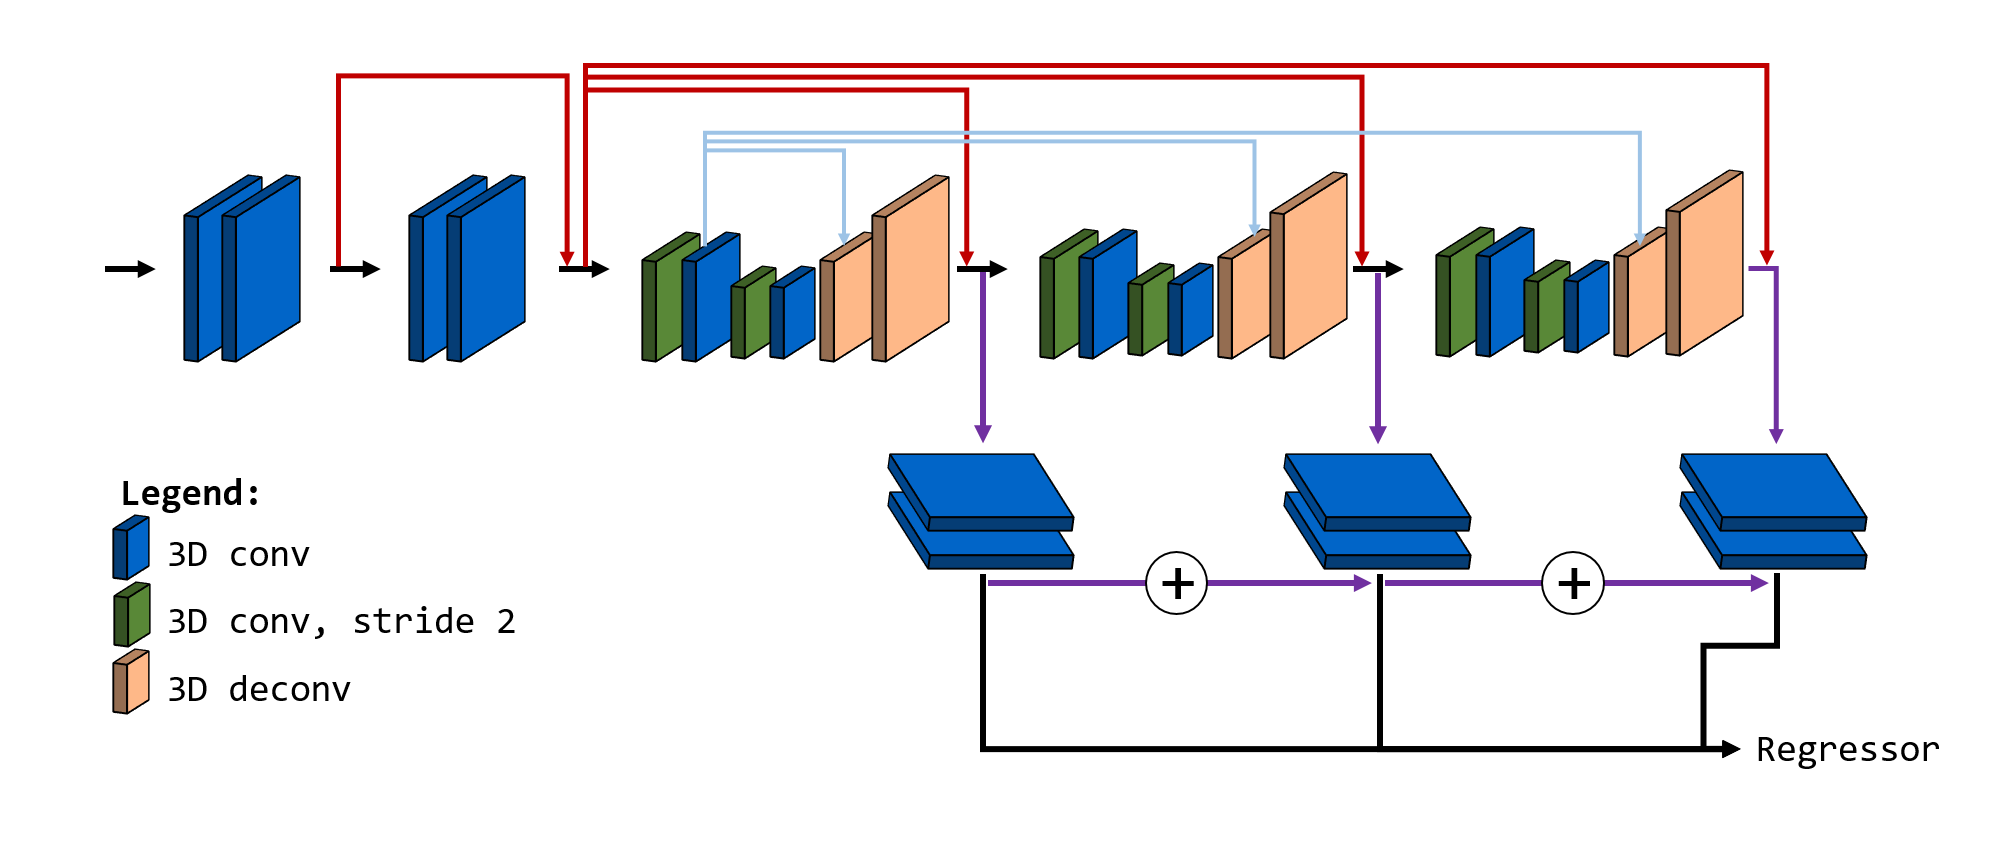
\includegraphics[width=0.9\linewidth]{Stacked Hourglass Architecture.png}
    \caption{Stacked hourglass.}
    \label{Fig:Stacked_hourglass}
\end{figure}
As already mentioned in section \ref{Sec:Joint_Processing}, our baseline model's residual 3D CNN for joint processing of cost volumes is abnormally shallow. Nevertheless, it would be naïve to append many further blocks without consideration, as this can be expected to aggravate the training process. However we are committed to improving learning of context features at this stage, and therefore seize the elegant solution presented by Chang and Chen \cite{PSM-Net}. They propose a \textit{stacked hourglass} 3D convolution architecture, as shown in figure \ref{Fig:Stacked_hourglass}, which is distinguished by three encoder-decoder like 3D CNNs extensively connected by skip connections. Each of these produce an output which is mapped by two layers of 3D convolutions to a volume of disparity scores, each of which can be converted to a disparity estimate by the regressor. This views the final stage of the network as a refinement process, as each subsequent identically constructed hourglass in essence only proposes a residual which corrects the previous estimates. This way, the training loss can be applied after each hourglass, a concept called \textit{intermediate supervision}. This facilitates and promotes incorporating local features at this stage rather than during the feature extraction at the head of the pipeline. We implement our version exactly according to the outline given in \cite{PSM-Net}, but do not want to list the multitude of individual input and output channel numbers here. The specifics are exhaustively documented in our code base, where we have implemented this component in completely unrolled fashion for legibility. 

\subsection{Putting it all together}
Recombining the aforementioned components is trivial, as they share very similar signatures with their templates in the baseline model. The only slight deviation is represented by the additional residual blocks required to provide the correct format for the cost volume creation, as described in section \ref{Sec:Gwc}. Overall, we obtain a model that ended up looking very similar to GwcNet \cite{guo2019groupwise}, although we adopted the stacked hourglass from PSM-Net \cite{PSM-Net} before finding the group-wise correlation volumes. However, GwcNet modifies the stacked hourglass by treating the intermediate outputs as independent, rather than passing them upwards to be modified by residuals. This speeds up inference, as intermediate estimates no longer need to be fully calculated, but from our point of view, it changes the style of this module significantly. We decide to retain this aspect in our model. In this respect, we point out the successful application of learned residuals to refine images in other tasks, for example compression artifact removal \cite{CompressionArtifactRemoval}. Finally, GwcNet concatenates a number of the final feature channels of a ResNet shared for left and right frames, while we obtain our feature maps using the feature fusion technique described in section \ref{Sec:Feature_Fusion}. For this reason, but also to explicitly acknowledge the extent of congruence with GwcNet, we refer to our improved version of the baseline model as \textbf{F}eature \textbf{F}usion GwcNet (FF-GwcNet).

\section{Experiments}
Our experiments seek to evaluate the performance of FF-GwcNet compared to the baseline model, the impact of different encoder types and stages in the feature fusion module. Also, we examine aspects of the training procedure, namely utilization of pretraining and aggressive data augmentation. All experiments used an Intel i9-9900K CPU paired with an RTX 3090 GPU.

\subsection{Datasets and Criteria}
In our pretraining experiments, we used the Scene Flow data set \cite{SceneFlow}, which contains $39\,824$ rendered images with dimensions $(H, W)=(540, 960)$. It features dense ground truth for disparity estimation and is subdivided into the different contexts. The first is \textit{Monkaa}, comprising $8\,664$ samples depicting a fantastical landscape, sometimes showing a strange blue creature. Next, there is \textit{Driving}, featuring rendered traffic scenes of a fictional city in $4\,400$ samples. Finally, the largest subset is \textit{FlyingThings3D}, which contains $26\,760$ very cluttered renderings of various objects at various scales. For FlyingThings3D, the authors provide a list containing allegedly unreasonably difficult samples, which we remove to obtain $26\,066$ samples in this subset, totaling $39\,130$ samples for the whole data set. While official training and testing splits exist, we are only concerned with this data set for the purpose of pretraining, so we instead randomly assign $80 \%$ of the samples to our training and the remainder to validation set. For all subsets, we use the \textit{finalpass} rendering quality.

For fine-tuning and then evaluating our models, the benchmark selected in the lab is the KITTI-2015 stereo disparity data set \cite{KITTI2015}, which contains $200$ real traffic scenes with sparsely annotated ground truth. The intended testing set ground truth is not publicly available, so we randomly split the data into $150$ training and $50$ testing samples. The image resolutions differs slightly between different samples. Here, we use the \textit{disp\_noc\_0} ground truth disparities.

Finally, we also considered the Cityscapes data set \cite{Cityscapes} for pretraining. However, the ground truth for the disparity task is annotated automatically for real traffic scenes, and seems rather noisy at first glance. Therefore, we decided not to use these samples.

The loss used for both pretraining and training is the smooth L1 loss
\begin{equation}
    \operatorname{SmoothL1} = \frac{1}{N} \sum_{i=1}^N l_i
\end{equation}
with
\begin{equation}
    l_i(X ,\hat{X}) = \begin{cases}
0.5(X_i - \hat{X}_i)^2 &|X_i - \hat{X}_i| \leq 1\\
|X_i - \hat{X}_i|-0.5 &\text{else}.
\end{cases}
\end{equation}
When FF-GwcNet is trained with intermediate supervision, the loss is applied relative to each estimate with the weights $\lambda = (0.5, 0.7, 1.0)$, the largest term corresponding to the final output. For evaluation, we additionally consider the 3-pixel error (3PE), given by
\begin{equation}
    \operatorname{3PE}(X ,\hat{X}) = 1 - \frac{1}{N} \sum_{i=1}^N \operatorname{CorrectDisp}(X_i - \hat{X}_i)
\end{equation}
where 
\begin{equation}
    \operatorname{CorrectDisp}(X_i, \hat{X}_i) = \begin{cases}
1 &|X_i - \hat{X}_i| < 3\\
1 &|X_i - \hat{X}_i| < 0.05 X_i\\
0 &\text{else}.
\end{cases}
\end{equation}
as well as analogously defined 1- and 5-pixel errors.

\subsection{Data Augmentation}
Data augmentation is not straightforward for disparity estimation, as most operations applied to the images must have a sensible counterpart for the disparity map. For example, we attempted to apply MixUp \cite{MixUp}, which blends several input samples and targets. However, a convex combination of disparity values does not make sense, so the training processes were not promising. In other cases, data augmentation is simply not compatible with the geometry of stereo camera rigs. This was true for random horizontal flips, which would have required exchanging left and right frames, flipping them, but then also converting the disparity such that it is relative to the former right frame. This is not possible in regions of the scene where the images do not overlap. Since KITTI-2015 is extremely small, we decided to apply a very aggressive augmentation by using CutMix \cite{CutMix}, which randomly crops other training samples into the ones shown to the model, replacing the same regions in the disparity map. In our core experiments, this is the only data augmentation used, as we are interested in a pure ablation of its utility in this context.

\subsection{Pretraining}
Pretraining was completed entirely on the Scene Flow data set for \textit{efficientnet-b3} and \textit{mobilenet\_v2} encoder backbones (the inconsistent names stemming from arguments in SMP). These were selected to obtain values for one fairly heavy and one very small encoder. This was combined with encoder depths of $3$ and $4$ for a total of four experiments using FF-GwcNet. In addition, the baseline model was also pretrained. In all cases, training starts with three epochs of warm-up, wherein the samples from Scene Flow are randomly cropped to $(512,928)$ and downsampled by a factor of two. The disparity is likewise downsampled and weighted with $0.5$ to adjust it to the scale of the pixel coordinate system. Finally, training is completed using two epochs of samples cropped to $(528, 944)$. The slight difference in input sizes is based on the circumstance that FF-GwcNet can only accept input sizes divisible by $16$ (that is $32$ for the downsampled warm-up epochs). One additional pretraining session with eight epochs was conducted to investigate whether pretraining for a longer time would have significant effects. Training and validation batch sizes were $(8,32)$ and $(2,8)$ for warm-up and full resolution training, respectively. Pretraining uses an Adam optimizer, the learning rate is reset to $0.001$ at the start of warm-up and full resolution training, and decayed each epoch by $0.6$ and $0.75$ respectively.

\subsection{Training}
Fine-tuning and evaluation was carried out on KITTI-2015 using \textit{efficientnet-b3} and \textit{mobilenet\_v2} backbones, but the encoder depth was fixed at $4$ following first insights from the pretraining experiments. Both models, as well as the baseline model, were trained using all four combinations of using or not using data augmentation or pretrained weights, which is a total of $12$ experiments. For the training set, the samples are randomly cropped to $(256,512)$ with batch sizes of $8$. For validation, a batch size of $1$ is used due to the irregular spatial dimensions of the images. Samples are reshaped to $(368, 1248)$ via bicubic interpolation, passed through the model and the disparity estimate is then interpolated back to the original shape. The output disparity is then weighted by $\frac{W_{\text{target}}}{1248}$ to account for the rescaling of the pixel coordinate system. Finally, all losses are evaluated with the respect to the sparse target, but only valid disparities counted. All training runs are constrained to run for a maximum of $240$ epochs, or stopped when the smooth L1 function on the validation set fails to improve for 24 epochs. The initial learning rate of $0.001$ is decayed by $0.992$ each epoch, the optimizer is also based on Adam.

\section{Results}
\subsection{Pretraining Results}
\begin{table}[h!]
\centering
\begin{tabular}{|l|l||l|l|l|l|l|}
\hline
\multicolumn{1}{|c|}{Encoder Backbone} & Encoder Depth & smoothL1       & 3PE              & 5PE             & 1PE              & \#params      \\ \hline\hline
\textit{efficientnet-b3}               & 3             & 1.275          & 0.08373          & 0.07208         & 0.1088           & 16M           \\
\textit{efficientnet-b3}               & 4             & {\ul 1.219}    & {\ul 0.07826}    & {\ul 0.06801}   & {\ul 0.1056}     & 16.7M         \\
\textit{mobilenet\_v2}                 & 3             & 1.383          & 0.08598          & 0.07379         & 0.1152           & {\ul 7.4M}    \\
\textit{mobilenet\_v2}                 & 4             & 1.345          & 0.08504          & 0.07334         & 0.1179           & 7.9M          \\
\textit{efficientnet-b3+Epochs}        & 4             & \textbf{1.001} & \textbf{0.07141} & \textbf{0.0627} & \textbf{0.08873} & 16.7M         \\
\textit{baseline model}                & -             & 2.23           & 0.1248           & 0.1084          & 0.1561           & \textbf{179k} \\ \hline
\end{tabular}
\caption{Pretraining Results.\label{Tab:Pretraining}}
\end{table}

Summarized in table \ref{Tab:Pretraining}, pretraining reveals a slight benefit to utilizing an encoder depth of $4$, which we deem worthwhile as it comes at a comparatively low cost. The baseline model is outperformed significantly, either in terms of its capabilities or of its learning speed, but has much fewer parameters than all other models. It should be noted that most parameters are contained in the feature fusion component, for example 12.7M for the deeper \textit{efficientnet-b3} variant. Also the \textit{efficientnet-b3} based encoder backbones perform better than their counterparts using \textit{mobilenet\_v2}, but comparable scores indicate that a variety of backbones should be capable of functioning within our framework. However, the performance on KITTI-2015 is of course the deciding factor, so we do not want to finalize such conclusions at this point. Our experiment with increasing the number of training epochs clearly yields some returns, but they are diminishing compared to the time invested. Figure \ref{Fig:Pretrain_Examples} shows one output each model for a sample from the validation set. Further insight into these experiments is provided in our corresponding WandB \cite{wandb} project\footnote{\url{https://wandb.ai/jannogga/CudaLab_SS21_Pretraining?workspace=user-jannogga}}.

\begin{figure}[t]
     \centering
     \begin{subfigure}[h]{0.32\linewidth}
         \centering
        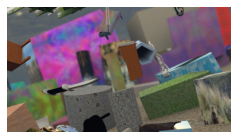
\includegraphics[width=\linewidth]{images/left_image_sceneflow.png}
        \caption{Left frame}
     \end{subfigure}
     \hfill
     \begin{subfigure}[h]{0.32\linewidth}
         \centering
        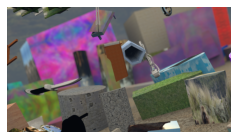
\includegraphics[width=\linewidth]{images/right_image_sceneflow.png}
        \caption{Right frame}
     \end{subfigure}
     \hfill
     \begin{subfigure}[h]{0.32\linewidth}
         \centering
        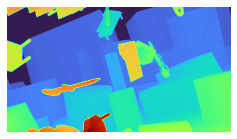
\includegraphics[width=\linewidth]{gt_sceneflow.png}
        \caption{Ground truth}
     \end{subfigure}
     \hfill
     \begin{subfigure}[h]{0.32\linewidth}
         \centering
        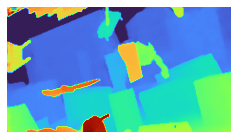
\includegraphics[width=\linewidth]{images/baseline_model_sceneflow.png}
        \caption{\textit{baseline model}}
     \end{subfigure}
     \hfill
     \begin{subfigure}[h]{0.32\linewidth}
         \centering
         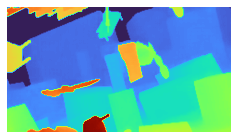
\includegraphics[width=\linewidth]{images/mobilenet_v2_sceneflow.png}
         \caption{\textit{mobilenet\_v2}}
     \end{subfigure}
          \hfill
    \begin{subfigure}[h]{0.32\linewidth}
         \centering
         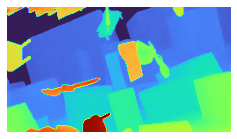
\includegraphics[width=\linewidth]{images/efficientnet-b3_sceneflow.png}
         \caption{\textit{efficientnet-b3}}
     \end{subfigure}
     \caption{An example image pair from the validation set of Scene Flow together with the target and predictions from each model. \label{Fig:Pretrain_Examples}}
\end{figure}


\subsection{KITTI-2015 Results}
\begin{figure}[h]
     \centering
     \begin{subfigure}[h]{0.32\linewidth}
         \centering
        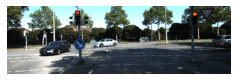
\includegraphics[width=\linewidth]{images/left_image_kitti.png}
        \caption{Left frame}
     \end{subfigure}
     \hfill
     \begin{subfigure}[h]{0.32\linewidth}
         \centering
        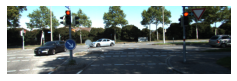
\includegraphics[width=\linewidth]{images/right_image_kitti.png}
        \caption{Right frame}
     \end{subfigure}
     \hfill
     \begin{subfigure}[h]{0.32\linewidth}
         \centering
        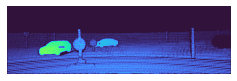
\includegraphics[width=\linewidth]{images/gt_kitti.png}
        \caption{Sparse ground truth}
     \end{subfigure}
     \hfill
     \begin{subfigure}[h]{0.32\linewidth}
         \centering
        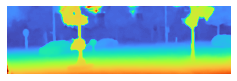
\includegraphics[width=\linewidth]{images/baseline_kitti_alt.png}
        \caption{\textit{baseline model}}
     \end{subfigure}
     \hfill
     \begin{subfigure}[h]{0.32\linewidth}
         \centering
         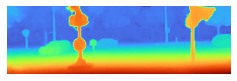
\includegraphics[width=\linewidth]{images/mobilenet_v2_kitti.png}
         \textit{mobilenet\_v2}
     \end{subfigure}
          \hfill
    \begin{subfigure}[h]{0.32\linewidth}
         \centering
         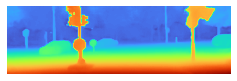
\includegraphics[width=\linewidth]{images/efficientnet-b3_kitti.png}
         \textit{efficientnet-b3}
     \end{subfigure}
     \caption{An example image pair from the validation set of KITTI-2015 together with the target and predictions from each model. \label{Fig:Finetune_Examples}}
\end{figure}

\begin{table}[h]
\centering
\begin{tabular}{|l|l|l||l|l|l|l|l|}
\hline
Encoder                 &             & Data         &                &                  &                 &                  & 3PE         \\
Backbone                & Pretraining & Augmentation & smoothL1       & 3PE              & 5PE             & 1PE              &  Zero-Shot \\ \hline\hline
\textit{efficientnet-b3}               & Yes         & Yes               & {\ul 0.428}    & \textbf{0.01791} & {\ul 0.01119}   & {\ul 0.07639}    & \textbf{0.07225}\\
                                       & Yes         & No                & \textbf{0.412} & {\ul 0.01813}    & \textbf{0.01097}& \textbf{0.06821} & \textbf{0.07225}\\
                                       & No          & Yes               & 0.484          & 0.02382          & 0.01433         & 0.0843           & 0.999         \\
                                       & No          & No                & 0.488          & 0.02279          & 0.0138          & 0.08558          & 0.999         \\ \hline
\textit{mobilenet\_v2}                 & Yes         & Yes               & 0.464          & 0.01985          & 0.01198         & 0.08873          & {\ul 0.129}   \\
                                       & Yes         & No                & 0.450          & 0.02018          & 0.01166         & 0.08419          & {\ul 0.129}   \\
                                       & No          & Yes               & 2.937          & 0.3503           & 0.1907          & 0.5862           & 0.999         \\
                                       & No          & No                & 0.602          & 0.02887          & 0.01771         & 0.1023           & 0.999         \\ \hline
\textit{baseline model}                & Yes         & Yes               & 0.553          & 0.03061          & 0.01753         & 0.1047           & 0.2834        \\
                                       & Yes         & No                & 0.544          & 0.03052          & 0.01673         & 0.1066           & 0.2834        \\
                                       & No          & Yes               & 0.809          & 0.05407          & 0.03162         & 0.1586           & 0.999         \\
                                       & No          & No                & 0.725          & 0.04657          & 0.02686         & 0.1403           & 0.999         \\ \hline
\end{tabular}
\caption{Training results.\label{Tab:Training}}
\vspace{-10pt}
\end{table}
The results of our ablation study on KITTI-2015 are summarized in table \ref{Tab:Training}. Pretraining can significantly improve the final performance of the each model. Successful transfer learning from Scene Flow to KITTI is further supported low zero-shot scores for pretrained models. Beyond the benefit visible in the table, training times were also much shorter for pretrained models. 

However, data augmentation using CutMix did not improve, but may even diminish the performance of the models without pretraining. For example the \textit{baseline model} in this scenario performs worse with data augmentation, and the training process for \textit{mobilenet\_v2} is hindered. In fact, it fails to reach the minimum required smooth L1 loss as defined in the lab sessions during its allotted training time. We believe it is plausible that CutMix introduces discontinuities in the disparity map which contradict the already learned features of the intersected object. This might challenge the model in an undesirable manner. All in all, such data augmentation may be too aggressive. We recommend using less aggressive forms, such as color jitter.

One further takeaway is that our improved model indeed achieves much better scores than the baseline version, validating the changes made. However, the baseline model also outperforms the lab requirements by a significant margin. In applications with reduced computational resources, its usage would be appropriate. Qualitative results from this experiment are shown in figure \ref{Fig:Finetune_Examples}. To appreciate the advantage of using an \textit{efficientnet-b3} backbone compared to a \textit{mobilenet\_v2} backbone, pay attention to the traffic light on the left of the image. The casing is captured in greater detail by the larger model. This is also reflected in the significant difference in 1PE scores between both versions. All of these results can be explored in the corresponding WandB-project\footnote{\url{https://wandb.ai/jannogga/CudaLab_SS21?workspace=user-jannogga}}.

\section{Outlook}
\begin{figure}[h]
     \centering
     \begin{subfigure}[h]{0.32\linewidth}
         \centering
        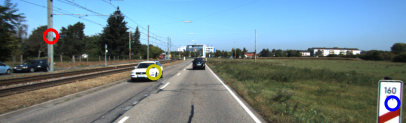
\includegraphics[width=\linewidth]{images/saliency_reference.png}
        \caption{Input image with three marked locations.}
     \end{subfigure}
     \hfill
     \begin{subfigure}[h]{0.32\linewidth}
         \centering
        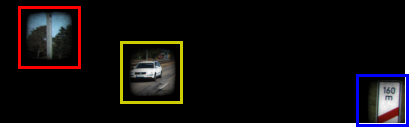
\includegraphics[width=\linewidth]{images/saliency_annotated_baseline.png}
        \caption{Saliency map for the \textit{baseline model}.}
     \end{subfigure}
     \hfill
     \begin{subfigure}[h]{0.32\linewidth}
         \centering
        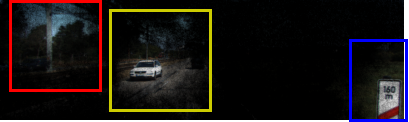
\includegraphics[width=\linewidth]{images/saliency_annotated_efficientnet-b3.png}
        \caption{Saliency map for the \textit{efficientnet-b3} FF-GwcNet.}
     \end{subfigure}
     \caption{Visualization of the combined saliency for selected regions of interest in an image pair.\label{Fig:Saliency}}
\end{figure}
Our experiments did not explore several interesting questions. Foremost, as mentioned in the previous section, other forms of data augmentation were not evaluated due to our interest in CutMix specifically.

While the overall improvement of the pipeline using our modifications is clear, the contributions of the individual changes are not. In this regard, further ablation studies that mix and match components of FF-GwcNet and the baseline model would be illuminating. Also, we cannot fully confirm that our stacked hourglass learns to consider the local context at a specific spatial location when determining the disparity. Our preliminary results using saliency maps, depicted in figure \ref{Fig:Saliency}, only demonstrate a larger effective field of view for the hourglass model. Other work, such as \cite{Cost_Volume}, relates this to the ability of their model to incorporate contextual information. We would not go so far, but agree that this aspect should be analyzed. 

Another issue is that the ground truth given for samples in KITTI-2015 lack annotations for the sky regions, because of physical limitations of the utilized sensors. In several images, the sky regions are assigned arbitrary values by our models, even though they were properly processed on Scene Flow. Some form of forgetting seems to occur here, which we could perhaps counteract by retaining some images from Scene Flow when fine-tuning on KITTI-2015.

With respect to our original goal of extending the perceptive capabilities of a humanoid robot, we regret that we could not obtain a fully pretrained segmentation model in an adequate form. Given this, we could fully freeze the feature fusion and evaluate training performance under these conditions. This would confirm whether FF-GwcNet can be integrated with existing vision systems as intended.

\section{Conclusion}
We successfully implement the proposed baseline model, train it to outperform the required specifications and further improved every trainable submodule of it. For training, we leverage a large synthetic data set, demonstrating the transfer of capabilities for all models tested. The results obtained using this training scheme for our FF-GwcNet are nearly perfect, boasting 3-pixel errors under $2 \%$. At the same time, the feature extraction was designed in a way that usage on top of an existing U-Net based segmentation system should be possible, at least from a structural perspective.

\section{Contributions}
Having access to powerful GPUs and buying Colab Pro for prototyping the models on the fly, Jan wrote most of the code. Unfortunately, the free version of Colab only rarely provided GPU-accelerated sessions and was thus not useful. We tried to compensate this issue as much as possible, reviewing the code in many meetings and also writing some parts together while discussing them. The contents and structure of the report was equally contributed to by both of us, and Fabrice created the figures.


% # Input: B x 64 x Disp/4 x H/4 x W/4
% # 2x conv3d 
% #-- 64->32 B x 32 x Disp/4 x H/4 x W/4
% # 2x conv3d
% #-- 32->32 B x 32 x Disp/4 x H/4 x W/4

% ## hourglass 1 
% # 1x downconv + 1x conv (downconv = 'strided 3D convolution')
% #-- 32->64 B x 64 x Disp/8 x H/8 x W/8
% # 1x downconv + 1x conv
% #-- 64->64 B x 64 x Disp/16 x H/16 x W/16
% # 2x convtranspose
% #-- 64->64 B x 64 x Disp/8 x H/8 x W/8
% #-- 64->32 B x 32 x Disp/4 x H/4 x W/4 -> c1

% ## hourglass 2
% # 1x downconv + 1x conv
% #-- 32->64 B x 64 x Disp/8 x H/8 x W/8
% # 1x downconv + 1x conv
% #-- 64->64 B x 64 x Disp/16 x H/16 x W/16
% # 2x convtranspose
% #-- 64->64 B x 64 x Disp/8 x H/8 x W/8
% #-- 64->32 B x 32 x Disp/4 x H/4 x W/4 -> c2

% ## hourglass 3
% # 1x downconv + 1x conv
% #-- 32->64 B x 64 x Disp/8 x H/8 x W/8
% # 1x downconv + 1x conv
% #-- 64->64 64 x Disp/16 x H/16 x W/16
% # 2x convtranspose
% #-- 64->64 B x 64 x Disp/8 x H/8 x W/8
% #-- 64->32 B x 32 x Disp/4 x H/4 x W/4 -> c3

% c1 #-- 32->1 B x 1 x Disp/4 x H/4 x W/4
% c2 #-- 32->1 B x 1 x Disp/4 x H/4 x W/4
% c3 #-- 32->1 B x 1 x Disp/4 x H/4 x W/4
% ---- Bibliography ----
\bibliographystyle{plain}  % we recommend the plain bibliography style
\bibliography{referencesAngel}       % xampl.bib comes with BibTeX
\end{document}
